\documentclass[preprint,12pt]{elsarticle}
\usepackage{amsmath,amssymb}
\usepackage{array,url}
\usepackage{tikz}
\usetikzlibrary{arrows.meta}

\begin{document}

\section*{Abstract}

\section*{Keywords}

\section*{Nomenclature}

\section{Introduction}
\label{sec:introduction}

\subsection{Background and Motivation}

\subsection{Related Work and Research Gaps}

\subsection{Contributions}

\section{Microgrid Modeling and Cooperative Scheduling Formulation}
\label{sec:formulation}

\subsection{System Architecture and Agent Responsibilities}
\label{sec:architecture}

Community $\mathcal{N}=\{1,\ldots,N\}$ comprises heterogeneous microgrids
with fixed loads, photovoltaic (PV) generation, a dispatchable generator (DG),
and a battery energy storage system (BESS) (Fig.~\ref{fig:community-architecture}).
Agents control generator/battery powers every $\Delta t=1$~h,
with $T=24$ steps per trajectory. A capacity-limited bus exchanges surplus;
the main grid supplies deficits. Grid export and load shedding are excluded.
The three-agent profiles are synthetic allocations preserving aggregate
hourly load/PV totals.
Scenario units are kW, kWh, and currency units per kWh (CU/kWh).

\begin{figure}[htbp]
 \centering
 \resizebox{\linewidth}{!}{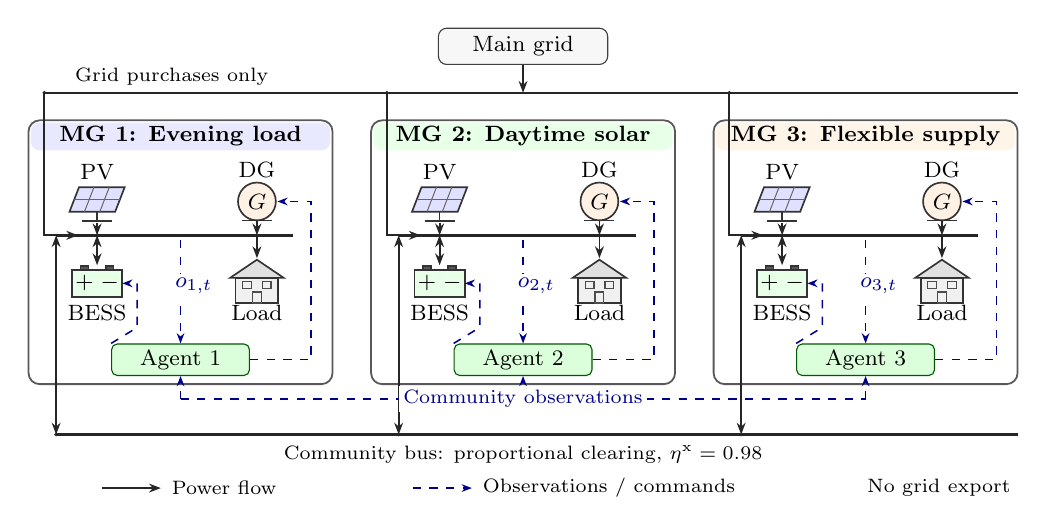
\begin{tikzpicture}[
 x=1cm,y=1cm,
 font=\fontsize{8}{9}\selectfont,
 power/.style={draw=black!85,line width=0.65pt,-{Stealth[length=1.5mm]}},
 exchange/.style={draw=black!85,line width=0.65pt,
   {Stealth[length=1.5mm]}-{Stealth[length=1.5mm]}},
 signal/.style={draw=blue!55!black,line width=0.55pt,dashed,
   -{Stealth[length=1.3mm]}},
 equipment/.style={draw=black!80,line width=0.6pt,fill=white},
 every node/.style={inner sep=1.5pt},
 pics/pv/.style={code={
   \draw[equipment,fill=blue!12] (-.35,-.13)--(.23,-.13)--(.35,.18)--(-.23,.18)--cycle;
   \draw[black!60,line width=.35pt]
     (-.29,.025)--(.29,.025)
     (-.16,-.13)--(-.04,.18)
     (.035,-.13)--(.155,.18);
   \draw[black!80,line width=.5pt] (0,-.13)--(0,-.25) (-.19,-.25)--(.19,-.25);
 }},
 pics/generator/.style={code={
   \draw[equipment,fill=orange!10] (0,0) circle[radius=.24];
   \node at (0,0) {$G$};
   \draw[black!80,line width=.5pt] (-.19,-.24)--(.19,-.24);
 }},
 pics/battery/.style={code={
   \draw[equipment,fill=green!9] (-.32,-.17) rectangle (.32,.17);
   \draw[equipment,fill=black!65] (-.21,.17) rectangle (-.11,.22);
   \draw[equipment,fill=black!65] (.11,.17) rectangle (.21,.22);
   \node at (-.16,0) {$+$};
   \node at (.16,0) {$-$};
 }},
 pics/load/.style={code={
   \draw[equipment,fill=black!6] (-.27,-.2) rectangle (.27,.12);
   \draw[equipment,fill=black!12] (-.34,.12)--(0,.35)--(.34,.12)--cycle;
   \draw[black!70,line width=.45pt] (-.18,-.02) rectangle (-.07,.07);
   \draw[black!70,line width=.45pt] (.07,-.02) rectangle (.18,.07);
   \draw[black!70,line width=.45pt] (-.055,-.2) rectangle (.055,-.06);
 }}
]
 \node[draw=black!75,rounded corners=3pt,fill=black!3,
   minimum width=2.15cm,minimum height=.46cm] (grid) at (6.4,5.47)
   {Main grid};
 \draw[black!85,line width=.85pt] (.32,4.88)--(12.68,4.88);
 \draw[power] (grid.south)--(6.4,4.88);
 \node[anchor=west,font=\fontsize{7}{8}\selectfont,fill=white]
   at (.65,5.08) {Grid purchases only};

 \foreach \offset/\agent/\role/\tint in {
   0/1/Evening load/blue,
   4.35/2/Daytime solar/green,
   8.70/3/Flexible supply/orange}{
   \begin{scope}[shift={(\offset,0)}]
     \draw[draw=black!65,line width=.65pt,rounded corners=4pt]
       (.12,1.18) rectangle (3.98,4.53);
     \path[fill=\tint!9,rounded corners=3pt] (.15,4.15) rectangle (3.95,4.50);
     \node[font=\fontsize{8}{9}\selectfont\bfseries] at (2.05,4.33)
       {MG \agent: \role};

     \pic at (.99,3.50) {pv};
     \pic at (3.02,3.50) {generator};
     \node[anchor=south] at (.99,3.72) {PV};
     \node[anchor=south] at (3.02,3.75) {DG};
     \draw[power] (.99,3.23)--(.99,3.07);
     \draw[power] (3.02,3.25)--(3.02,3.07);
     \draw[black!85,line width=1.1pt] (.47,3.07)--(3.48,3.07);
     \draw[power] (.32,4.88)--(.32,3.07)--(.75,3.07);
     \fill[black!85] (.32,4.88) circle[radius=.025];

     \pic at (.99,2.46) {battery};
     \pic at (3.02,2.41) {load};
     \node at (.99,2.08) {BESS};
     \node at (3.02,2.08) {Load};
     \draw[exchange] (.99,3.07)--(.99,2.69);
     \draw[power] (3.02,3.07)--(3.02,2.78);

     \node[draw=green!35!black,fill=green!14,rounded corners=2pt,
       minimum width=1.75cm,minimum height=.40cm] (agent\agent) at (2.05,1.49)
       {Agent \agent};
     \draw[signal] (2.05,3.01)--(agent\agent.north);
     \node[text=blue!55!black,fill=white] at (2.22,2.43) {$o_{\agent,t}$};
     \draw[signal] (agent\agent.north west)--(1.5,1.90)--(1.5,2.46)--(1.31,2.46);
     \draw[signal] (agent\agent.east)--(3.71,1.49)--(3.71,3.50)--(3.28,3.50);
     \draw[exchange] (.47,3.07)--(.47,.54);
     \fill[black!85] (.47,.54) circle[radius=.025];
     \draw[signal] (2.05,.99)--(agent\agent.south);
   \end{scope}
 }

 \draw[blue!55!black,line width=.55pt,dashed] (2.05,.99)--(10.75,.99);
 \node[text=blue!55!black,fill=white,font=\fontsize{7}{8}\selectfont]
   at (6.4,.99) {Community observations};
 \draw[black!85,line width=.85pt] (.47,.54)--(12.68,.54);
 \node[font=\fontsize{7}{8}\selectfont] at (6.4,.29)
   {Community bus: proportional clearing, $\eta^{\mathrm{x}}=0.98$};

 \draw[power] (1.05,-.14)--(1.80,-.14);
 \node[anchor=west,font=\fontsize{7}{8}\selectfont] at (1.88,-.14) {Power flow};
 \draw[signal] (5.0,-.14)--(5.75,-.14);
 \node[anchor=west,font=\fontsize{7}{8}\selectfont] at (5.83,-.14)
   {Observations / commands};
 \node[anchor=east,font=\fontsize{7}{8}\selectfont] at (12.65,-.14)
   {No grid export};
\end{tikzpicture}
}
 \caption{Microgrid community. Solid lines denote power flows; blue dashed
 lines denote observations and dispatch commands.}
 \label{fig:community-architecture}
\end{figure}

\subsection{Component Models and Operational Constraints}
\label{sec:components}

Generator output $p_{i,t}^{\mathrm{g}}$ lies between zero and its rating
$\overline{P}_i^{\mathrm{g}}$. Let $z_{i,t}$ denote battery state of charge
(SOC), $E_i$ its rated energy, and $\eta_i^{\mathrm{ch}}$,
$\eta_i^{\mathrm{dis}}$ its charging/discharging efficiencies.
Battery power $p_{i,t}^{\mathrm{b}}$ is positive for discharge.
With $[x]^+=\max(x,0)$, SOC evolves as
\begin{equation}
 z_{i,t+1}=z_{i,t}
 -\frac{[p_{i,t}^{\mathrm{b}}]^+\Delta t}{\eta_i^{\mathrm{dis}}E_i}
 +\frac{\eta_i^{\mathrm{ch}}[-p_{i,t}^{\mathrm{b}}]^+\Delta t}{E_i}.
 \label{eq:soc-transition}
\end{equation}

For lower/upper SOC bounds $\underline{z},\overline{z}$ and rated powers
$\overline{P}_i^{\mathrm{ch}},\overline{P}_i^{\mathrm{dis}}$,
the available charging/discharging limits are
\begin{equation}
 \begin{aligned}
 \overline{p}_{i,t}^{\mathrm{ch}}
 &=\min\left\{\overline{P}_i^{\mathrm{ch}},
       \frac{(\overline{z}-z_{i,t})E_i}
            {\eta_i^{\mathrm{ch}}\Delta t}\right\},\\
 \overline{p}_{i,t}^{\mathrm{dis}}
 &=\min\left\{\overline{P}_i^{\mathrm{dis}},
       \frac{(z_{i,t}-\underline{z})E_i\eta_i^{\mathrm{dis}}}
            {\Delta t}\right\}.
 \end{aligned}
 \label{eq:battery-limits}
\end{equation}

Thus $-\overline{p}_{i,t}^{\mathrm{ch}}\leq p_{i,t}^{\mathrm{b}}
\leq\overline{p}_{i,t}^{\mathrm{dis}}$. SOC continues across days.

For load $L_{i,t}$, available PV power $V_{i,t}$, and exchange limit
$\overline{P}_i^{\mathrm{x}}$, residual demand and transferable
supply/demand are
\begin{gather}
 n_{i,t}=L_{i,t}-V_{i,t}-p_{i,t}^{\mathrm{g}}-p_{i,t}^{\mathrm{b}},
 \label{eq:residual-demand}\\
 u_{i,t}=\min\{[-n_{i,t}]^+,\overline{P}_i^{\mathrm{x}}\},\qquad
 v_{i,t}=\min\{[n_{i,t}]^+,\overline{P}_i^{\mathrm{x}}\}.
 \label{eq:exchange-offers}
\end{gather}

Total supply $U_t=\sum_i u_{i,t}$ and demand $D_t=\sum_i v_{i,t}$,
with delivery efficiency $\eta^{\mathrm{x}}$, give proportional clearing:
\begin{equation}
 \begin{aligned}
 F_t&=\min\{U_t,D_t/\eta^{\mathrm{x}}\},\\
 p_{i,t}^{\mathrm{send}}&=u_{i,t}F_t/U_t,\qquad
 p_{i,t}^{\mathrm{recv}}=v_{i,t}\eta^{\mathrm{x}}F_t/D_t .
 \end{aligned}
 \label{eq:proportional-exchange}
\end{equation}

Here $F_t$ is total power sent before losses;
$p_{i,t}^{\mathrm{send}},p_{i,t}^{\mathrm{recv}}$ are local sent/received
powers. Transfers are zero when $U_tD_t=0$ and use only residual surplus.

\subsection{Scheduling Objective and Energy Balance}
\label{sec:objective}

Grid purchase power $p_{i,t}^{\mathrm{grid}}$ and unused surplus power
$p_{i,t}^{\mathrm{spill}}$ satisfy
\begin{equation}
 p_{i,t}^{\mathrm{grid}}=[n_{i,t}-p_{i,t}^{\mathrm{recv}}]^+,\qquad
 p_{i,t}^{\mathrm{spill}}=[-n_{i,t}-p_{i,t}^{\mathrm{send}}]^+.
 \label{eq:grid-spill}
\end{equation}

The local power balance is
\begin{equation}
 V_{i,t}+p_{i,t}^{\mathrm{g}}+p_{i,t}^{\mathrm{b}}
       +p_{i,t}^{\mathrm{grid}}+p_{i,t}^{\mathrm{recv}}
 =L_{i,t}+p_{i,t}^{\mathrm{send}}+p_{i,t}^{\mathrm{spill}}.
 \label{eq:power-balance}
\end{equation}

Surplus can include excess DG output. For purchase tariff $\lambda_t>0$,
economic and full costs are
\begin{align}
 C_{i,t}^{\mathrm{econ}}&=\big[
 \lambda_t p_{i,t}^{\mathrm{grid}}
 +a_i(p_{i,t}^{\mathrm{g}})^2+b_i p_{i,t}^{\mathrm{g}}+c_i
 +k_i^{\mathrm{b}}|p_{i,t}^{\mathrm{b}}|
 +k^{\mathrm{x}}p_{i,t}^{\mathrm{send}}\big]\Delta t,
 \label{eq:economic-cost}\\
 C_{i,t}&=C_{i,t}^{\mathrm{econ}}
              +\epsilon_i p_{i,t}^{\mathrm{g}}\Delta t.
 \label{eq:full-cost}
\end{align}

Here $a_i,b_i,c_i$ are quadratic, linear, and constant generator-cost
coefficients ($c_i=0$); $k_i^{\mathrm{b}}$ prices battery energy throughput
and $k^{\mathrm{x}}$ prices energy sent. The coefficient $\epsilon_i$
is the generator environmental-cost proxy in CU/kWh.

Over operating horizon $\mathcal{H}$, minimize expected community cost:
\begin{equation}
 \min_{\boldsymbol{\pi}}\;
 \mathbb{E}_{\boldsymbol{\pi}}
 \left[\sum_{t\in\mathcal{H}}\sum_{i\in\mathcal{N}}C_{i,t}\right],
 \label{eq:dispatch-objective}
\end{equation}
subject to the modeled constraints. Here $\boldsymbol{\pi}=(\pi_1,\ldots,\pi_N)$
collects local dispatch policies, and $\mathbb{E}_{\boldsymbol{\pi}}$
averages over their operating trajectories.

\subsection{Cooperative Sequential Decision Formulation}
\label{sec:decision}

The partially observable state comprises SOCs and the exogenous sequence
position. Observations $o_{i,t}\in\mathbb R^{20}$ combine local measurements,
equipment/time features, forecasts, and community broadcasts;
\ref{sec:observation-appendix} defines their components.
Causal forecasts use published tariffs and
training-only load/PV templates. Centralized training uses joint
observations
$s_t^{\mathrm{c}}=\operatorname{concat}(o_{1,t},\ldots,o_{N,t})
\in\mathbb R^{20N}$.

Actions $a_{i,t}=(a_{i,t}^{\mathrm{g}},a_{i,t}^{\mathrm{b}})
\in[0,1]\times[-1,1]$ map to power as
\begin{equation}
 p_{i,t}^{\mathrm{g}}=a_{i,t}^{\mathrm{g}}\overline P_i^{\mathrm{g}},
 \qquad
 p_{i,t}^{\mathrm{b}}=[a_{i,t}^{\mathrm{b}}]^+\overline p_{i,t}^{\mathrm{dis}}
 -[-a_{i,t}^{\mathrm{b}}]^+\overline p_{i,t}^{\mathrm{ch}}.
 \label{eq:action-mapping}
\end{equation}

Here $a_{i,t}^{\mathrm{g}}$ is the generator loading fraction;
$a_{i,t}^{\mathrm{b}}$ is the signed available battery-power fraction,
positive for discharge and negative for charging.

All agents receive the common reward
\begin{equation}
 r_t=\frac{\kappa}{N}\sum_i(C_{i,t}^{0}-C_{i,t}),\qquad
 J_\gamma(\boldsymbol{\pi})=
 \mathbb{E}_{\boldsymbol{\pi}}\left[\sum_{k=0}^{\infty}\gamma^k r_k\right],
 \label{eq:team-reward}
\end{equation}

Here $\kappa=0.1$ is the reward scale, $\gamma=0.99$ the
discount factor, $J_\gamma$ expected discounted return, and $k$ the
time-step index. Reference $C_{i,t}^{0}$ uses zero generator and battery
powers under identical data and clearing. The reward retains discounted-cost
rankings; reported costs are undiscounted~\eqref{eq:dispatch-objective}.


\section{Evolution-Enhanced Graph-Attentive Cooperative Scheduling}
\label{sec:method}

\subsection{Framework and Dispatch Interface}
\label{sec:method-framework}
\label{sec:dispatch-interface}

Battery inventory couples dispatch across hours. Community exchange
couples microgrid costs. Graph-Attentive Value
Decomposition Actor-Critic (GAVDAC) uses recurrent histories to condition
community-value estimation and an evolutionary algorithm (EA) to explore
complete dispatch policies. Its policy-gradient backbone follows Factored
Multi-Agent Centralised Policy Gradients (FACMAC)~\cite{facmac2021};
graph mixing builds on GraphMIX~\cite{graphmix2020}, and population
interaction follows evolutionary reinforcement learning (ERL)~\cite{erl2018}.

Figure~\ref{fig:method-framework} shows the two learning branches.
The actor, local critic, and mixer have parameters $\theta$, $\phi$, and
$\psi$, respectively. A population of $M$ complete shared actors supplies
additional trajectories to replay buffer $\mathcal D$. Gradient learning
updates $(\theta,\phi,\psi)$; selection, mutation, and actor injection
update the population.

\begin{figure}[htbp]
 \centering
 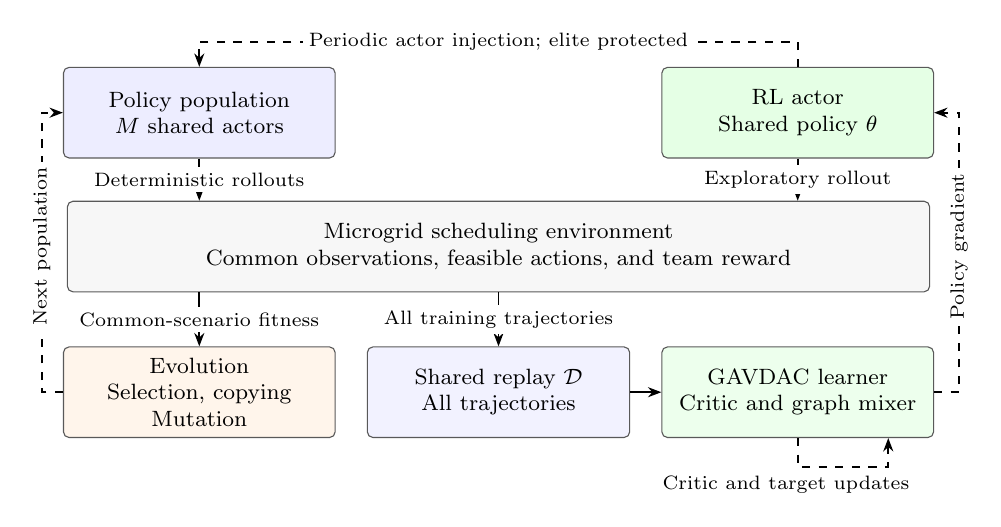
\begin{tikzpicture}[
 x=1cm,y=1cm,
 font=\footnotesize,
 block/.style={draw=black!65,rounded corners=2pt,align=center,
   text width=3.05cm,minimum height=1.15cm,inner sep=4pt},
 flow/.style={-{Stealth[length=1.7mm]},line width=.65pt},
 update/.style={flow,dashed},
 lab/.style={font=\scriptsize,fill=white,inner sep=2pt,align=center}
]
 \node[block,fill=blue!7,minimum width=3.45cm] (pop) at (1.9,4.25)
   {Policy population\\$M$ shared actors};
 \node[block,fill=green!10,minimum width=3.45cm] (actor) at (9.5,4.25)
   {RL actor\\Shared policy $\theta$};
 \node[block,fill=black!3,text width=10.65cm,minimum width=10.95cm] (env) at (5.7,2.55)
   {Microgrid scheduling environment\\
    Common observations, feasible actions, and team reward};
 \node[block,fill=orange!8,minimum width=3.45cm] (evo) at (1.9,.70)
   {Evolution\\Selection, copying\\Mutation};
 \node[block,fill=blue!5,minimum width=3.25cm] (replay) at (5.7,.70)
   {Shared replay $\mathcal{D}$\\All trajectories};
 \node[block,fill=green!7,minimum width=3.45cm] (learner) at (9.5,.70)
   {GAVDAC learner\\Critic and graph mixer};

 \draw[flow] (pop.south)--(env.north -| pop.south)
   node[midway,lab] {Deterministic rollouts};
 \draw[flow] (actor.south)--(env.north -| actor.south)
   node[midway,lab] {Exploratory rollout};
 \draw[flow] (env.south)--(replay.north)
   node[midway,lab] {All training trajectories};
 \draw[flow] (replay.east)--(learner.west);
 \draw[flow] (env.south -| evo.north)--(evo.north)
   node[midway,lab] {Common-scenario fitness};

 \draw[update] (evo.west)--(-.10,.70)--(-.10,4.25)--(pop.west);
 \node[lab,rotate=90] at (-.10,2.55) {Next population};
 \draw[update] (learner.east)--(11.55,.70)--(11.55,4.25)--(actor.east);
 \node[lab,rotate=90] at (11.55,2.55) {Policy gradient};
 \draw[update] (actor.north)--(9.5,5.15)--(1.9,5.15)--(pop.north);
 \node[lab] at (5.7,5.15) {Periodic actor injection; elite protected};
 \draw[update] (learner.south)--(9.5,-.25)--(10.65,-.25)--(learner.south -| 10.65,0);
 \node[lab] at (9.35,-.48) {Critic and target updates};
\end{tikzpicture}

 \caption{Population exploration and graph-attentive learning. Solid arrows
 carry policies, actions, or experience; dashed arrows denote updates.}
 \label{fig:method-framework}
\end{figure}

Each agent receives local measurements, equipment limits, community
broadcasts, and causal forecast summaries as defined in
Section~\ref{sec:decision}. Its generator and battery coordinates pass
through Eq.~\eqref{eq:action-mapping}. Scaling battery actions by available
charging/discharging power exposes the feasible flexibility as SOC changes.
The centered reward retains the discounted-cost ranking of policies on
a common operating sequence. Exchange clearing and grid balancing follow
Section~\ref{sec:formulation}.

\subsection{History-Conditioned Graph Value Decomposition}
\label{sec:graph-decomposition}

The shared actor receives $[o_{i,t},a_{i,t-1},e_i]$, where $e_i$ is a
one-hot agent identifier. An input layer with a rectified linear unit (ReLU)
and a gated recurrent unit (GRU) produce hidden state $h_{i,t}$.
A linear output with a hyperbolic tangent gives the two-component vector
$\nu_{i,t}\in[-1,1]^2$, affinely mapped to action bounds
$[0,1]\times[-1,1]$. Parameters are shared, while observations,
identifiers, and hidden states distinguish microgrid roles.

A local critic gives utility $q_{i,t}=q_\phi(o_{i,t},a_{i,t})$.
History features are $\zeta_{i,t}=\operatorname{ReLU}(W_hh_{i,t}+b_h)$.
Attention scores are
$u_{ij,t}=(W_Q\zeta_{i,t})^\top(W_K\zeta_{j,t})/\sqrt{d_\zeta}$.
Here $W_h,b_h,W_Q,W_K$ are trainable projections and $d_\zeta$ is the
query/key dimension. For binary mask $C$, normalized weights are
\begin{equation}
 A_{ij,t}=\frac{C_{ij}\exp(u_{ij,t})}
                    {\sum_{k=1}^{N}C_{ik}\exp(u_{ik,t})}.
 \label{eq:mixer-attention}
\end{equation}

The implemented mask is
$C=\left[\begin{smallmatrix}1&1&1\\1&1&0\\1&0&1\end{smallmatrix}\right]$.
It defines utility-aggregation connections independently of physical
exchange links. Attention varies within this fixed mask as histories evolve.

For utility vector $q_t=(q_{1,t},\ldots,q_{N,t})^\top$, the mixed team
value is
\begin{equation}
 \begin{aligned}
 f_{i,t}&=g_\psi\big((A_tq_t)_i;s_t^{\mathrm{c}}\big),\\
 Q_{\mathrm{tot},t}
 &=\left(\frac1N\sum_i f_{i,t}\right)
          w_{\mathrm{out}}(s_t^{\mathrm{c}})+V(s_t^{\mathrm{c}}).
 \end{aligned}
 \label{eq:graph-value}
\end{equation}

The graph transformation $g_\psi$ applies two state-conditioned affine
layers with leaky ReLU and exponential linear unit activations.
The vector $f_{i,t}$ is the resulting node feature,
$w_{\mathrm{out}}$ weights its mean readout, and $V$ is a scalar bias.
These functions use the layer-normalized joint observation
$s_t^{\mathrm{c}}$. Hypernetworks generate nonnegative weights through
scaled sigmoids, following QMIX~\cite{qmix2018}. For fixed state and
recurrent features, the team value is nondecreasing in local utilities.
Actor histories thus condition both dispatch and community-value mixing.

\subsection{Joint-Value Policy Learning}
\label{sec:policy-learning}
\label{sec:facmac-learning}

Replay retains daily sequences to reconstruct recurrent histories.
Let $\tau_t$ denote joint replayed histories,
$\boldsymbol\mu_\theta$ the joint actor, and $\boldsymbol h_t^\theta$
its hidden states. Superscript $-$ denotes target networks.
For true-terminal indicator $d_t$, the bootstrap target is
\begin{equation}
 y_t=r_t+\gamma(1-d_t)Q_{\mathrm{tot}}^-
 \big(s_{t+1}^{\mathrm{c}},
      \boldsymbol\mu_{\theta^-}(\tau_{t+1}),\boldsymbol h_{t+1}^{-}\big).
 \label{eq:td-target}
\end{equation}

The critic and mixer minimize the mean squared target error over valid
transitions, with actor features detached. After this update, their
parameters are fixed while the actor minimizes
\begin{equation}
 \mathcal L_\pi(\theta)=
 -\left\langle Q_{\mathrm{tot}}
 (s_t^{\mathrm{c}},\boldsymbol\mu_\theta(\tau_t),\boldsymbol h_t^\theta)
 \right\rangle
 +\lambda_a\left\langle\|\nu_{i,t}\|_2^2/2\right\rangle.
 \label{eq:actor-loss}
\end{equation}

Angle brackets denote sample means, including agents for the action
regularizer with coefficient $\lambda_a$. Gradients pass through actions
and recurrent attention features. Target networks use soft parameter
updates after each learner update; settings appear in
Section~\ref{sec:experimental-setup}.

Previous actions in replay reconstruct both current and target histories.
Daily execution resets hidden states and previous actions, while SOC
continues across days. The final bootstrap extends the preceding history,
giving a blockwise approximation at the day boundary.

\subsection{Common-Scenario Evolution and Learning Interaction}
\label{sec:evolution}
\label{sec:hybrid-interaction}
\label{sec:training-procedure}

At each EA cycle, all $M$ candidates use deterministic actions on the same
training day with the same initial SOC vector. Candidate $k$ receives
fitness $F_k=\sum_{t=0}^{T-1}r_t^{(k)}$, its undiscounted daily team return.
Matching exogenous inputs and initial energy makes within-cycle fitness
differences attributable to policy behavior.

Rank-based tournaments select policies while protecting the elite.
The configured crossover copies one paired complete actor into the other,
with a randomly chosen direction. Mutation perturbs selected matrix
weights using relative Gaussian noise, with occasional large perturbations
or resets; bias vectors remain unchanged. One evaluated generation updates
the complete shared actor per cycle. Operator settings are given in
Section~\ref{sec:experimental-setup}.

All population trajectories enter $\mathcal D$. The gradient actor then
collects a trajectory from the same scenario using ordinary exploration;
its final SOC and date advance training. After replay warmup, learner
updates proceed in critic/mixer, actor, and target order. The updated actor
is injected into a population slot chosen from pre-evolution fitness while
protecting the retained elite. Population experience therefore reaches the
learner through replay, and gradient-trained behavior reaches the population
through injection.

Every population rollout counts toward the interaction budget. Validation
trajectories are excluded from replay, and the actor and population elite
remain separate checkpoint candidates. Online scheduling uses only the
selected deterministic actor, recurrent states, and prescribed
measurements/broadcasts, followed by feasible-power mapping and exchange
clearing. The critic, mixer, and evolution operate during training.


\section{Case Studies}
\label{sec:case-studies}

\subsection{Experimental Setup}
\label{sec:experimental-setup}

The selected training configuration is
\texttt{facmac\_ea\_tune\_v03\_long}, combined with
\texttt{microgrid} and the shared defaults through the training entry point.
Table~\ref{tab:training-settings} records its settings.

\begin{table}[htbp]
 \centering
 \footnotesize
 \caption{Selected training and validation settings.}
 \label{tab:training-settings}
 \begin{tabular}{>{\raggedright\arraybackslash}p{0.62\linewidth}
                 >{\raggedright\arraybackslash}p{0.27\linewidth}}
 \hline
 Setting & Value\\
 \hline
 Training interaction budget & $6\times10^6$ steps\\
 Minibatch / replay capacity / warmup & 128 / 50,000 / 512 episodes\\
 Actor and local critic hidden width & 48\\
 Mixer / hypernetwork / attention width & 32 / 64 / 16\\
 Actor / critic learning rate & $3\times10^{-4}$ / $10^{-4}$\\
 Optimizer / gradient norm limit & Adam / 5\\
 Discount / soft target coefficient & 0.99 / 0.002\\
 Action regularization coefficient & $10^{-3}$\\
 Random-action period / Gaussian noise deviation & 1,000 steps / 0.05\\
 Population size / elite fraction & 5 / 0.2\\
 Mutation / copy-crossover probability & 0.9 / 1.0\\
 Large-mutation and reset probability (each) & 0.05\\
 Per-row mutated column fraction & 1.0\\
 EA start threshold / trigger interval & 10,000 steps / 5 iterations\\
 Generations / learner updates per EA cycle & 1 / 3\\
 Ordinary learner trigger / updates per trigger & 2 iterations / 1\\
 Validation interval / days & 10,000 steps / 8\\
 Validation initial SOC & 0.35\\
 Computation & CPU, float32\\
 \hline
 \end{tabular}
\end{table}

Validation uses the first eight validation days, with a common initial SOC
for each day and exploration disabled. RL and population checkpoints are
selected separately; the principal deployment policy is the
validation-selected RL actor. These daily-reset validation scores are
distinct from continuous-inventory operating-cost evaluation.


\subsection{Economic Performance and Operational Feasibility}

\subsection{Learning Efficiency and Training Stability}

\subsection{Ablation Studies}

\subsection{Generalization and Robustness}

\subsection{Coordinated Dispatch Behavior}

\section{Conclusions}
\label{sec:conclusions}

\appendix
\section{Observation and Forecast Definitions}
\label{sec:observation-appendix}

For $Y_{-i,t}=\sum_{j\ne i}Y_{j,t}$, define usable AC-side battery energy
$B_{i,t}=(z_{i,t}-\underline{z})E_i\eta_i^{\mathrm{dis}}$ and time phase
$\theta_t=2\pi h_t/24$, where $h_t$ is the current hour.
The 20 components of $o_{i,t}$ are listed in
Table~\ref{tab:observation-map}. Price, power, and energy scaling constants
are $S_\lambda=0.3$~CU/kWh, $S_P=300$~kW, and $S_E=1200$~kWh.
Scaling affects network inputs only.

\begin{table}[htbp]
 \centering
 \footnotesize
 \caption{Ordered observation components for agent $i$.}
 \label{tab:observation-map}
 \begin{tabular}{>{\raggedright\arraybackslash}p{0.09\linewidth}
                 >{\raggedright\arraybackslash}p{0.54\linewidth}
                 >{\raggedright\arraybackslash}p{0.22\linewidth}}
 \hline
 Entries & Physical quantities & Divisor\\
 \hline
 1 & Current tariff $\lambda_t$ & $S_\lambda$\\
 2--3 & Local load $L_{i,t}$ and PV power $V_{i,t}$ & $S_P$\\
 4 & SOC $z_{i,t}$ & 1\\
 5--6 & $\sin\theta_t,\cos\theta_t$ & 1\\
 7--8 & Other-agent totals $L_{-i,t},V_{-i,t}$ & $S_P$\\
 9 & Other-agent usable energy $B_{-i,t}$ & $S_E$\\
 10 & Generator rating $\overline{P}_i^{\mathrm{g}}$ & $S_P$\\
 11 & Battery capacity $E_i$ & $S_E$\\
 12 & Exchange limit $\overline{P}_i^{\mathrm{x}}$ & $S_P$\\
 13--14 & Available charge/discharge powers from
          Eq.~\eqref{eq:battery-limits} & $S_P$\\
 15--17 & Next tariff, next-$H$ mean tariff, next-$H$ maximum tariff
          & $S_\lambda$\\
 18--19 & Mean local forecasts
          $\widehat{L}_{i,t,H},\widehat{V}_{i,t,H}$ & $S_P$\\
 20 & Other-agent net forecast
          $\sum_{j\ne i}(\widehat{L}_{j,t,H}-\widehat{V}_{j,t,H})$
          & $S_P$\\
 \hline
 \end{tabular}
\end{table}

For $X\in\{L,V\}$, let $\mu_i^X(h)$ be the mean profile at hour $h$
over training days. The current-level multiplier is
$r_{i,t}^X=\operatorname{clip}(X_{i,t}/\mu_i^X(h_t),0.25,2)$
when $\mu_i^X(h_t)>10^{-8}$ and equals one otherwise.
The mean forecast over $H=4$ future hours is
\begin{equation}
 \widehat{X}_{i,t,H}=\frac{r_{i,t}^X}{H}
    \sum_{k=1}^{H}\mu_i^X((h_t+k)\bmod24).
 \label{eq:causal-forecast}
\end{equation}

Tariff summaries use the same future hours of the published daily tariff.
At midnight, template and tariff indices wrap to hour zero.
Neither forecast reads future realized load or PV from the evaluation day.


\bibliographystyle{../templates/elsarticle/elsarticle-num}
\bibliography{../bibliography}

\end{document}
